% Drawing 63/05-1 -- folder 63, batch 05, archive page 95 (PDF page 96).
% Transcription: En haut de la page, un dessin : une droite horizontale marquée $\Delta = 0$ ; plus bas une droite marquée « $j=0$ i.e.\ $c_4=0$ » et une courbe marquée « $j=12^3$ i.e.\ $c_6=0$ », qui la coupe en deux points, au-dessus de $p=2$ (à gauche) et de $p=3$ (à droite), reliés par des traits pointillés à une droite de base où ces deux points sont marqués. Légendes :
% Kind: moduli of elliptic curves over Spec Z: divisors j = 0, j = 12^3 above p = 2, 3. Method 2 (schematic redraw from the facsimile). Status: ok.
% Notes: A horizontal line Delta = 0 at the top; lower, the line j = 0 (c_4 = 0) and the curve j = 12^3 (c_6 = 0) meeting it in two points, above p = 2 (left) and p = 3 (right), joined by dashed verticals to a base line where both points are marked. The four legends (automorphism groups of order 24 and 12 with arrows to the two points; divisors of multiplicity 2 and 3 with ticks) are placed as on the page, their wording after the transcription.
% Coordinates: 1 unit = 1 mm = 1/100 of the crop width (bbox in page fractions: [0.08, 0.06, 0.6, 0.4]).
% Redrawn by Claude (claude-opus-5-5), issue #73, 2026-11-07; not checked by a human; not compiled (no TeX in the session).
% Rights: reproduces part of the work -- behind RENDER_TRANSCRIPTS, never published by itself.
\documentclass[tikz,border=3pt]{standalone}
\usepackage{amsmath,amssymb}
\usetikzlibrary{patterns,arrows.meta}
\tikzset{pencil/.style={black!45}, struck/.style={black!35}, mark/.style={circle,draw,inner sep=1.3pt}, pt/.style={circle,fill,inner sep=0.9pt}, opt/.style={circle,draw,fill=white,inner sep=1.1pt}}
\begin{document}
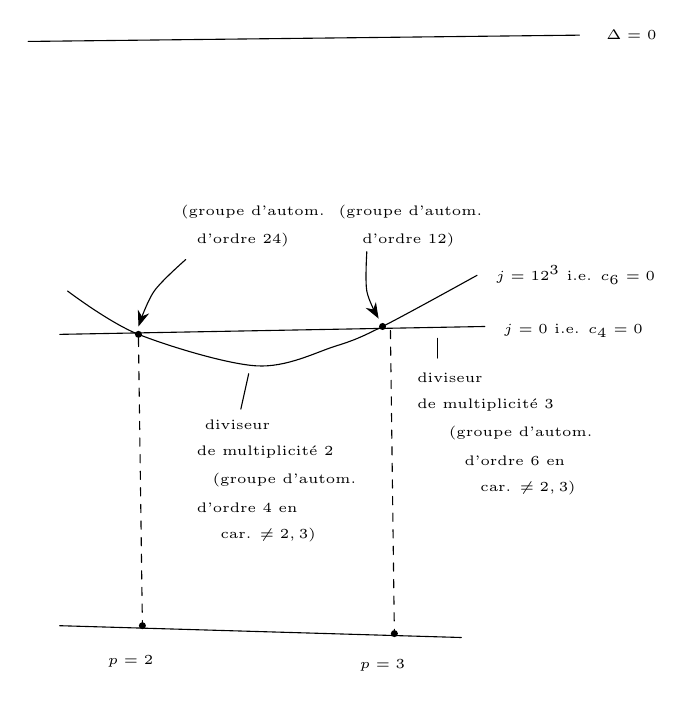
\begin{tikzpicture}[x=1mm,y=1mm,line cap=round,line join=round,font=\scriptsize]
\draw (19,-9.3) -- (89,-8.5);
\node[inner sep=1pt,anchor=west] at (92,-8.5) {\tiny $\Delta=0$};
\draw (23,-46.5) -- (77,-45.5);
\node[inner sep=1pt,anchor=west] at (79,-46) {\tiny $j=0$ i.e. $c_4=0$};
\draw plot[smooth, tension=0.55] coordinates {(24,-41) (33,-46.5) (48,-50.5) (58,-48) (64,-45.5) (76,-39)};
\node[inner sep=1pt,anchor=west] at (78,-39) {\tiny $j=12^3$ i.e. $c_6=0$};
\node[pt] at (33,-46.5) {};
\node[pt] at (64,-45.5) {};
\draw[dashed] (33,-47) -- (33.5,-83.5);
\draw[dashed] (65,-46) -- (65.5,-84.5);
\draw (23,-83.5) -- (74,-85);
\node[pt] at (33.5,-83.5) {};
\node[pt] at (65.5,-84.5) {};
\node[inner sep=1pt] at (32,-88) {\tiny $p=2$};
\node[inner sep=1pt] at (64,-88.5) {\tiny $p=3$};
\draw[-{Stealth[length=2mm]}] plot[smooth, tension=0.55] coordinates {(39,-37) (35,-41) (33,-45.5)};
\node[inner sep=1pt,anchor=west] at (38,-31) {\tiny (groupe d'autom.};
\node[inner sep=1pt,anchor=west] at (40,-34.5) {\tiny d'ordre 24)};
\draw[-{Stealth[length=2mm]}] plot[smooth, tension=0.55] coordinates {(62,-36) (62,-41) (63.5,-44.5)};
\node[inner sep=1pt,anchor=west] at (58,-31) {\tiny (groupe d'autom.};
\node[inner sep=1pt,anchor=west] at (61,-34.5) {\tiny d'ordre 12)};
\draw (47,-51.5) -- (46,-56);
\node[inner sep=1pt,anchor=west] at (41,-58) {\tiny diviseur};
\node[inner sep=1pt,anchor=west] at (40,-61.5) {\tiny de multiplicité 2};
\node[inner sep=1pt,anchor=west] at (42,-65) {\tiny (groupe d'autom.};
\node[inner sep=1pt,anchor=west] at (40,-68.5) {\tiny d'ordre 4 en};
\node[inner sep=1pt,anchor=west] at (43,-72) {\tiny car. $\neq 2,3$)};
\draw (71,-47) -- (71,-49.5);
\node[inner sep=1pt,anchor=west] at (68,-52) {\tiny diviseur};
\node[inner sep=1pt,anchor=west] at (68,-55.5) {\tiny de multiplicité 3};
\node[inner sep=1pt,anchor=west] at (72,-59) {\tiny (groupe d'autom.};
\node[inner sep=1pt,anchor=west] at (74,-62.5) {\tiny d'ordre 6 en};
\node[inner sep=1pt,anchor=west] at (76,-66) {\tiny car. $\neq 2,3$)};
\end{tikzpicture}
\end{document}
